\section{RIMA1 and RIMA2: Conditianal Assessment Robotic Tools for Sewer Pipes}

\label{sec:industry}

\textbf{Brief: } RIMA1 [~\ref{fig:rima1}] and RIMA2 [~\ref{fig:rima2}] are two robotic tools developed by the UTS Robotics Institute in collaboration with Sydney Water. They are designed to conditially assess the pipe walls of sewer 
pipes using Pulse Eddy Current (PEC) Sensors. Both robots operate in the ROS1 framework and are equipped with various sensors and cameras such as IMU and RGB-D cameras. Both robots communicate with the base station using VDSL via a 
kevlar braided cable. The subsections will go over more specific tasks I did on RIMA1 and RIMA2 meaning it will excluide things such as general maintenance and repair which was definitely done given these robtots are prototypes.

\begin{figure*}[htbp]
    \centering
    \begin{minipage}[t]{0.48\textwidth}
        \centering
        \includegraphics[width=\textwidth]{images/rima1/RIMA1_Physical_Weight_Detatched.jpg}
        \caption{RIMA1}
        \label{fig:rima1}
    \end{minipage}
    \hfill
    \begin{minipage}[t]{0.48\textwidth}
        \centering
        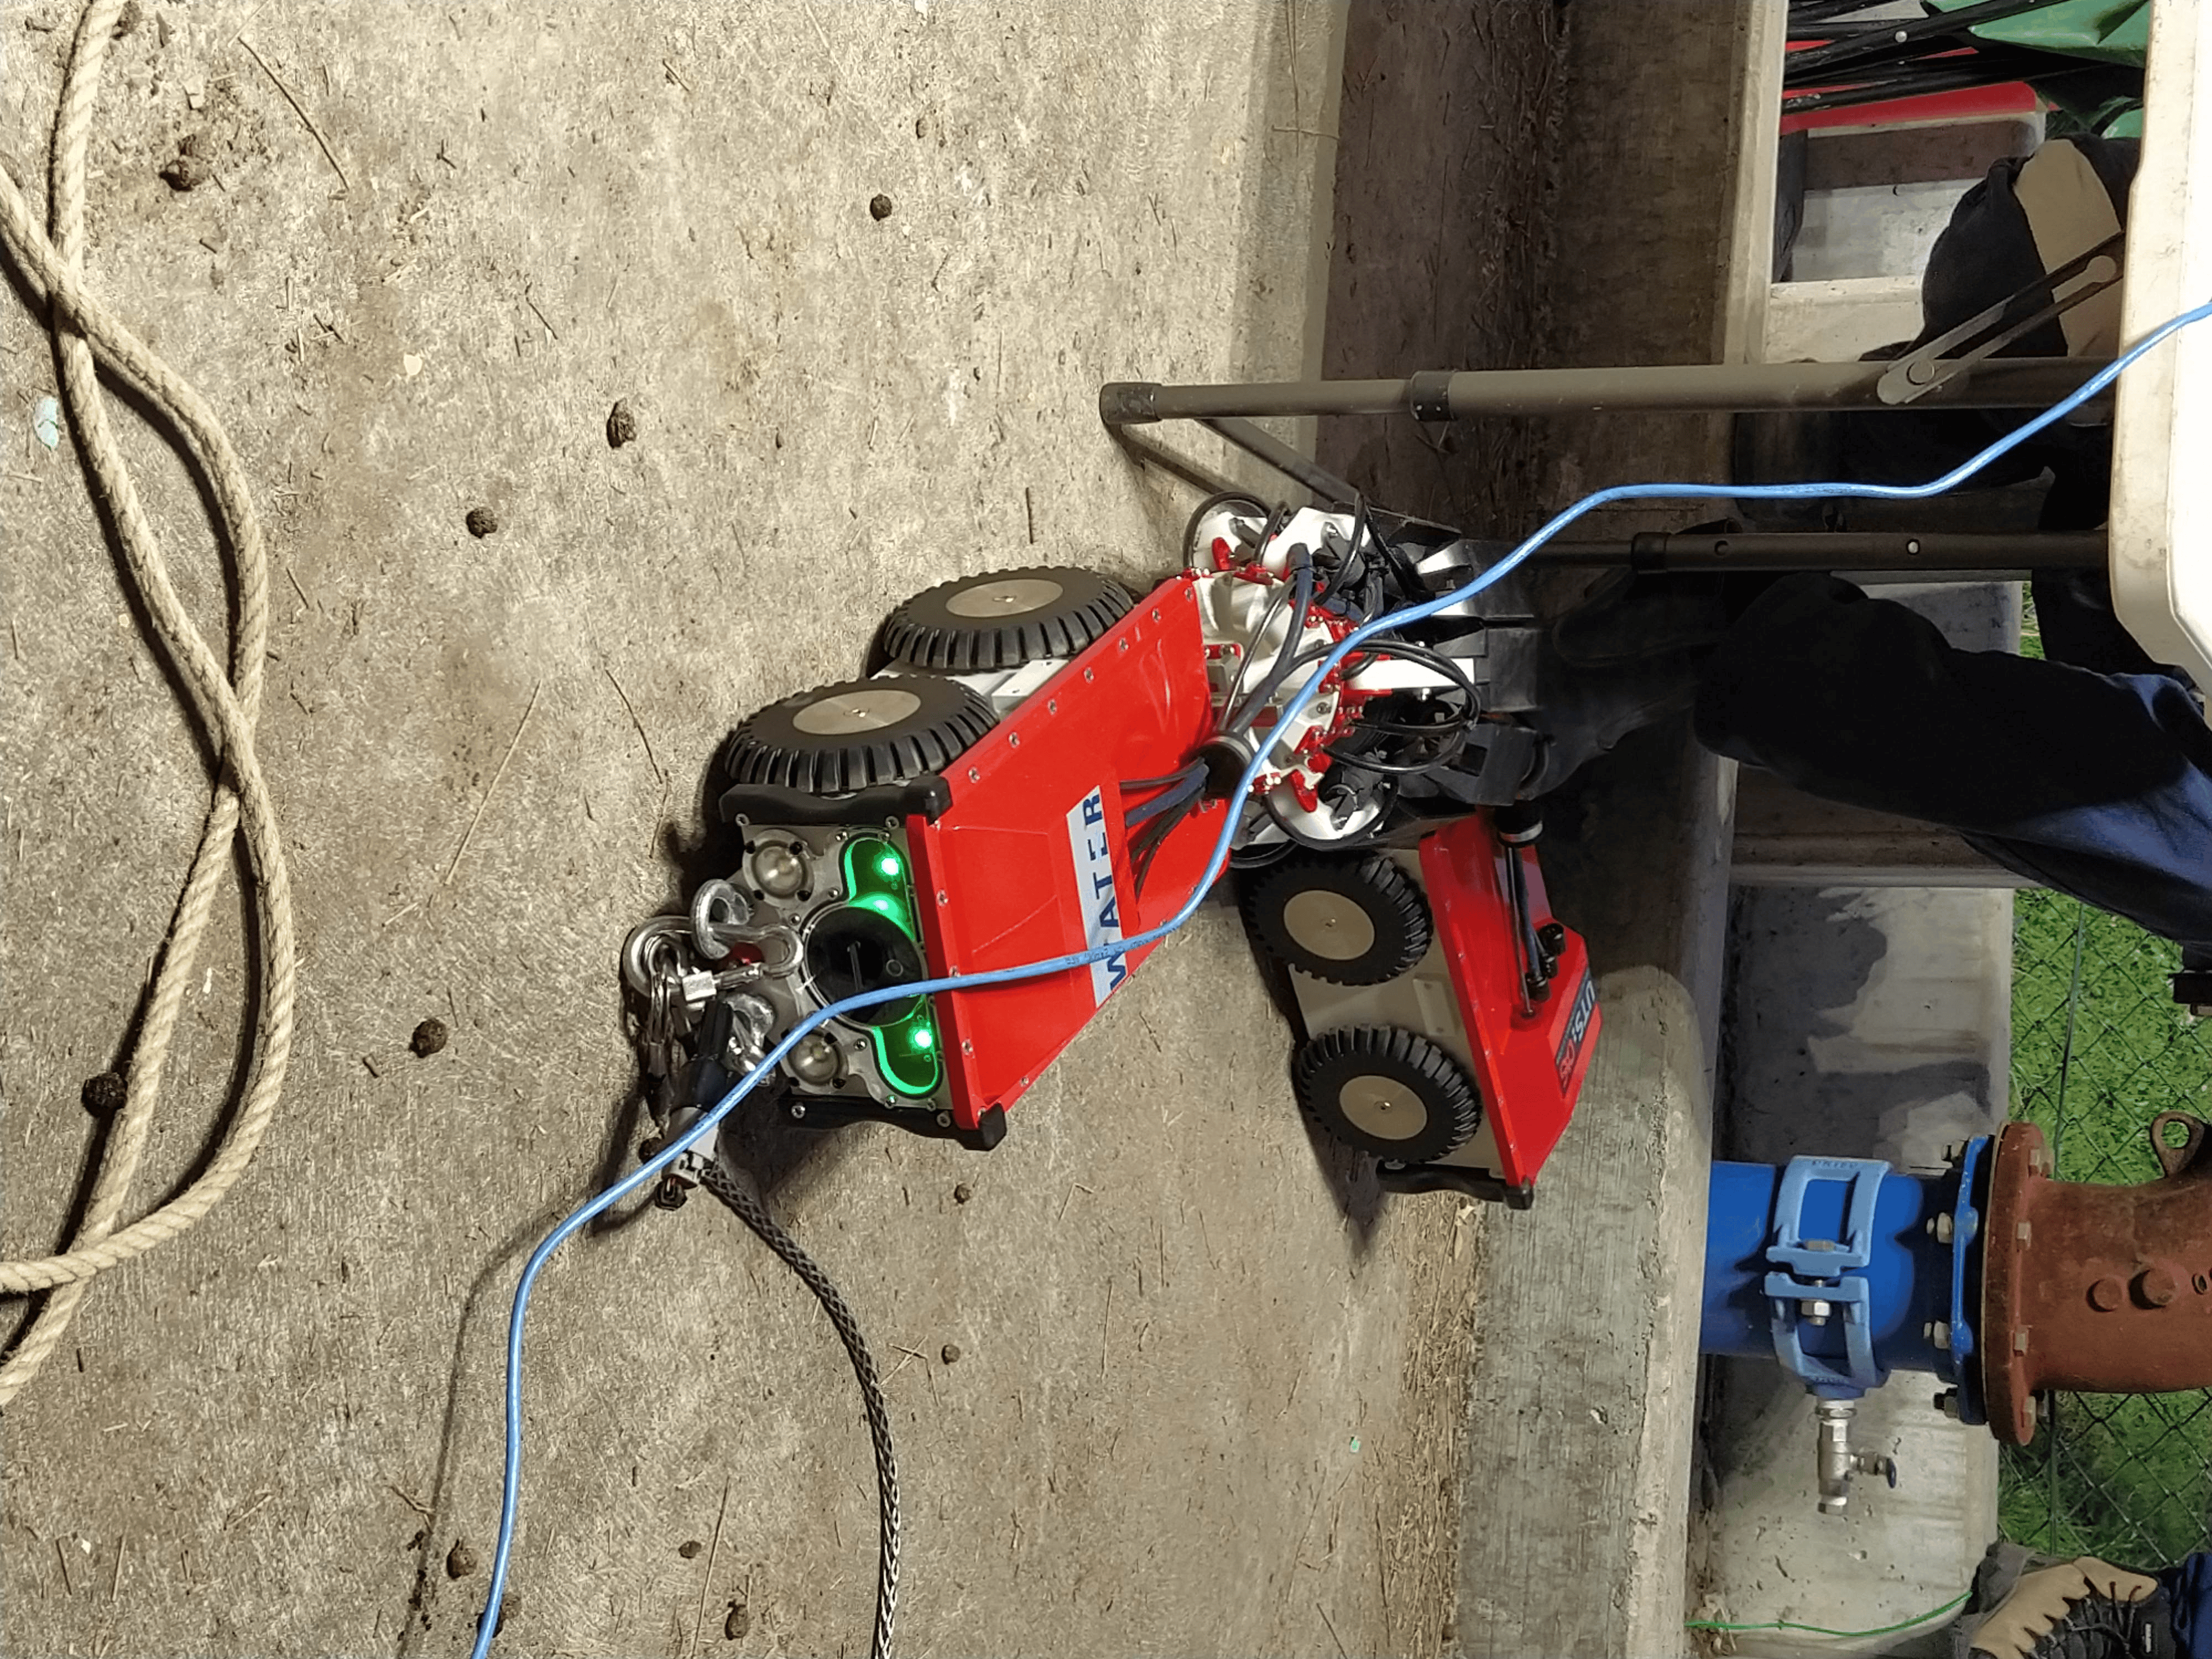
\includegraphics[angle=90, width=\textwidth]{images/rima2/RIMA2_Physical.png}
        \caption{RIMA2}
        \label{fig:rima2}
    \end{minipage}
\end{figure*}

% Tether Protetiion Section
\newpage
\subsection{Mechanical Work}

%\textbf{Utilities for RIMA1 and RIMA2 Field Trials:} 
\subsubsection{Utilities for RIMA1 and RIMA2 Field Trials:}
I designed a number of utilities to assist with field trial deployments to prevent damage to equipment and site. Using Solidworks I designed
tether protection for flangless and flanged pipes [~\ref{fig:tethproc}] which were later manufactured to be used in deployments. The tether protection units are designed with the following intent:

\begin{itemize}
    \item Ease of use for Sydney Water personnel
    \item Prevent damage to the tether and pipe wall at entrance where edge is sharp
    \item Adjustability for different pipe diameters (250mm to 750mm)
    \item Stainless steel for Chemical and Weather resitance and durability
    \item Simple lock-pin mechanism to ensure ease of use when wearing gloves
    \item Teflon block with internal radius matched to the bend radius of tether cable connected from base station to the robot
    \item Simple, low cost design
\end{itemize}

\imgpairin{utility/flangless_tether_protection.JPG}{Flangless Tether Protection}{utility/tether_protection_flanged.JPG}{Flanged tether protection}{Tether Protection}{tethproc}{90}{270}

% Deployment Cradle Section
\newpage
\subsubsection{RIMA2 Deployment Cradle:}
The next utility I designed was a deployment cradle for RIMA2 [~\ref{fig:jdm}]. Often, due to safety constraints only one person is allowed into the sewer pit. This does not favour the handling of RIMA2 which is a 3-body 
system best carried and inserted into pipes safely by two people. There was an incident during a field trial where RIMA2 was dropped, I was assigned with designing the cradle. The advantage 
of the cradle is that it can safely lower and deploy RIMA2. The final deisgn features:

\begin{itemize}
    \item Ability to be lowered using block-and-chain or cranes (varies with resource availability on site)
    \item Lightweight to ensure weight requirements are met as per agreement with Sydney Water
    \item Simple, intuitive locking mechanisms to ensure ease of use for Sydney Water personnel
    \item Custom flange design to adapt to various flanged pipe diameters (250mm to 450mm) if additional support is required
\end{itemize}

\imgpairin{utility/jdm.jpg}{RIMA2 Cradle in lab}{utility/jdm_in_use.jpg}{Cradle in use on field trial}{RIMA2 Cradle}{jdm}{0}{270}

% Rollover-Assist RIMA1
\newpage
%\textbf{RIMA1 Rollover Assist:} 
\subsubsection{RIMA1 Rollover Assist:}
I designed a set of rollover assist devices for RIMA1 after an incident in one of the first trial runs with Sydney Water during the handover period
a software bug caused the robot to drive autonomously up the pipe wall causing in to invert. The aim of the rollover assist is to help with manually pulling the robot out the pipe when it inverts, as 
using machinery to dig up the robot can be costly, time-consuming and potentially impossible depending on location.The inital inspiration [~\ref{fig:rp}] actually came from when I pulled apart my skateboard and attached it to RIMA1.
The final design [~\ref{fig:fdra}] after a few iterations is quite different from this and is simply a modification of the Sensor Pad on the sensor head with a custom bracket that could be fitted to RIMA1 with simple modification to the lifting handles.  

\imginin{rima1/rollover_prototype.jpg}{Rollover Prototype}{rp}{0.29}
\imgpairin{rima1/rollover_rear.jpg}{Rollover Assist Rear View}{rima1/rollover_side.jpg}{Rollover Side View}{Final Design Rollover Assist}{fdra}{270}{0}

\subsection{Electrical Work}

% RIMA1 System Board Instalation
%\textbf{RIMA1 System Board Installation:}
\subsubsection{RIMA1 System Board Installation:}
I installed a new system board on RIMA1 [~\ref{fig:sbi}] to fix in-rush current issues. This occured when the robot was turned on which caused a large in-rush and the battery BMS to kick in and turn off for safety and could not be reset without removing the lid of RIMA1 and 
unplugging the battery directly to reset. It also featured a new IMU which I made a simple vector normalisation algorithm for to ensure data was correct. The installation also required simple probing and electrical tests
to ensure it was working properly. 

\imgpairin{rima1/system_board_old.JPG}{Old System Board}{rima1/system_board_new.JPG}{New System Board}{System Board Installation}{sbi}{0}{0}

% RIMA2 New PEC Board Test Rig
%\textbf{RIMA2 New PEC Board Test Rig:}
\subsubsection{RIMA2 New PEC Board Test Rig:}
RIMA2 was to be fitted with a new PCB circuit which used Darlington Mosfets to drive the sensors instead op-amps used on by predecessor. This was to allow for stronger signal amplification which would allow reasonable signals to 
be picked up on pipe walls with thick concrete lining (> 20mm). To validate the Darlington Mosfet, I created a test rig for the chip which could be attached to the predecessor board.

\imginin{rima2/new_pec_test.jpg}{Darlington Mosfet Perf Board Setup}{newpec}{0.4}


% RIMA2 New PEC Board Installation
\newpage
%\textbf{RIMA2 New PEC Board Installation:}
\subsubsection{RIMA2 New PEC Board Installation:}
Once tests were validated. The teams senior engineer who works remotely designed the new PEC board and it was my task to install it [~\ref{fig:npi}]. This wasn't a simple installation as the receiver board (black PCB) had to be removed and remounted to 
where the old PEC board was mounted. This is becasue the Mosfets of the new board are quite large and clearence is needed to ensure it fits within the sensor head. Installing the board required 
hand soldering extremely small wires and SMD components that were damaged or fell off the recevier board when relocating. It also required soldering USB data lines to the new PEC board.

\imgpairin{rima2/pec_install_location.JPG}{New Pec to be installed ontop of Receiver Board}{rima2/pec_new_installed.JPG}{New PEC PCB}{New PEC System Installed}{npi}{0}{0}

% RIMA2 Debugging
%\textbf{RIMA2 Electrical Debugging:}
\subsubsection{RIMA2 Electrical Debugging:}

RIMA2 is a very small, compact robot and with that came many issues. Especially after the new PEC board was installed. Various debugging was completed on RIMA2 to ensure everything was working as intended and to fix any issued.
Debugging and fixes include:

\begin{itemize}
    \item Replacing PEC USB cable which became faulty due to strain during installation and earlier testing with the Sensor Head open
    \item USB voltage testing for rear cart camera which was no longer being detected. Other software based diagnosis such as dmesg was done for this issue as well. Camera cable was eventually replaced
    \item RIMA2 ran off and NVIDIA Jetson Xavier AGX. Port health was checked for PEC and Cameras.
    \item Probing of RIMA2 PEC and System Boards for debugging and diagnosis when PEC would arbitrarily stop working.
    \item Further PCB debugging to identify and replace faulty components such as regulators.
\end{itemize}
\newpage
\subsection{Software Work}

% Give a brief software overview
%\textbf{Software Brief: }
\subsubsection{Software Brief: }
RIMA1 and RIMA2 ran off the ROS1 Melodic framework. They utilised custom messages and customised ROS packages to function. All code for the robot was written in C++ and analysis scripts used for PEC are written
in Python. Unfortunately the codebases for these robots cannot be shared as it is property of UTS and Sydney Water. The robots processes and GUI's are all run/launched ushing shell scripts in the linux CL.

% New RIMA1 system board software update
\vspace{\baselineskip}
%\textbf{RIMA1 System Board Software Update: }
\subsubsection{RIMA1 System Board Software Update: }
The new system board required some minor software updates. This primarily consisted of changes to message data types and names. This change also required small modification to RIMA1's core.cpp file which was resposible 
for ROS handling (i.e. setting up subscribers, publishers, etc.). 

% RIMA1 GUI Update
\vspace{\baselineskip}
%\textbf{RIMA1 GUI Update: }
\subsubsection{RIMA1 GUI Update: }
The old GUI of RIMA was outdated and not greatly designed and doing something simple such as turning required going into settings and modifying rotation setpoints which is clearly not ideal or user friendly. I updated
the GUI [~\ref{fig:r1gui}] to have more intuitive control, I also installed rear cameras at the time for rear view and visual view of the sensor to have a better cue of full expansion rather than basing it off the current reading. Basic 
IMU visualisation was also added to the GUI to allow for better understanding of the robot's orientation in the pipe. The GUI was written in C++ using Qt Designer.

\begin{figure*}[htbp]
    \centering
    \subfloat[Old RIMA1 interface]{
        \includegraphics[width=0.30\textwidth, valign=c]{images/rima1/rima1_old_gui.jpg}
    }
    \hspace{0.5cm}
    \subfloat[New RIMA1 interface]{
        \includegraphics[width=0.60\textwidth, valign=c]{images/rima1/rima_gui_new.png}
    }
    \caption{Comparison of RIMA1 GUI's}
    \label{fig:r1gui}
\end{figure*}
\newpage
\imginin{rima1/rear_cam_rear.jpg}{RIMA1 Rear Camera rear View}{rcam}{0.8}

% Embedded software debugging for RIMA2 PEC
\subsubsection{RIMA2 PEC Embedded Software Debugging: }

When RIMA2's PEC Board was installed, its microcontroller onboard the PCD was also upgraded and used slightly different libraries compared to the old PCB for SPI communication. The way the Sensor Head has 10 PEC
channels that each have an ADC daisy-chained together. From a software standpoint the channels buffer through in a loop so all 10 channels are obtained and transferred via SPI. With the new MCU, Libary and PEC board,
10 inidvidual channels of data did not come through. Instead the 1st channel appeared to override all channels and there were 10 identical plots of data. After logic analysing and electrical debugging, if was found that 
the Chip Select was a consant and as a result, would not allow proper buffering through the ADCs. Once this was changed, PEC worked as expected.

% PEC Calibration
\newpage
\subsubsection{RIMA PEC Calibration: }
PEC was regularly calibrated before field trials to ensure that sensors were fully functional. PEC curves could be extracted and analysed [~\ref{fig:pecdata1}] [~\ref{fig:pecdata2}] using Python Scripts. 

\imginin{rima1/lo_0mm_th_all.png}{PEC data RIMA2 no concrete lining results}{pecdata1}{0.58}
\imginin{rima1/lo_11.54mm_th_all.png}{PEC data RIMA2 11.54mm concrete lining results}{pecdata2}{0.58}

% Simplified shell script for data tranfer and other stuff
\newpage
\subsubsection{Other Software Work:}

There were a few other software tasks I did such as creating new shell scripts for QOL such as easier data transfer between robot and base station. This made it more intuitve for anyone using to command line rather than having to memorise
shell copy commands. I was also in the process of creating a Master GUI in collaboration with our Senior Engineer. This was to make everything more user firendly for Sydney Water to grant them capability in having non-technical
staff operate the robots. However, due to project timeline constraints, whilst built, it was never tested fully.
   